\documentclass{article}

\usepackage{graphicx}

\title{Physical Controller Report}
\author{Harry Donovan - HD241610}
\date{https://drive.google.com/open?id=1I5zGk7EhjqBN9vi6QOgywfug1ZDW6TGo}

\begin{document}
    \maketitle

    \tableofcontents

    \newpage

    \section{Project Proposal}
        \subsection{Concept Overview}
            Humanity has been forced into underground bunkers. Automated production facilities ensure an endless bombardment of shells. You are a defence operator, tasked with controlling a defensive turret above the bunker. A majority of the systems are automated and require only limited guidance, with the system breaking the complex hail of debris and 3D trajectories into a more manageable 2D display. Keep us safe for as long as you can; our survival is in your hands.

        \subsection{Software Overview}
            The game is inspired by the classic arcade game missile defender. It is a 2D game in which you control the rotation of a turret which is able to fire up at incoming projectiles. The spawning of enemies is controlled by one of several AI modules, with the active module changing as the game progresses.The spawned enemies can take a variety of different AI modules and one is assigned at spawn by the spawn AI. These AI modules are ‘hot-swappable’, so I may experiment with the enemies AI changing mid wave. I also plan to implement special ‘Boss’ enemies, as well as enemies with unique abilities.

        \subsection{Hardware Overview}
            I will repurpose a Sony ST-SE500 FM-AM tuner for the controller. I chose this controller as it has the needed inputs, and makes sense in-universe as recycled and repurposed equipment. I also originally intend to use the vacuum fluorescent display, however due to how the display PCB is set up this is unfortunately unrealistic. The arduino will be stored within the case, with the cable connecting it to the PC running out of the cable port that was originally for the mains power supply. I plan to repurpose one of the push-to-make buttons and the rotary encoder.
    
    \newpage

    \section{The Controller}
        \subsection{Hardware}
            As stated in my proposal I will repurpose a Sony ST-SE500 Stereo/ FM-AM Tuner. I will be using the case in order to store the arduino, running the cable connecting the arduino to a PC through the cases' original power supply port. The rotary encoder and a single button are also on a separate PCB, so I have cut the wires that connected it to the main board and am instead running them into the arduino. The rotary encoder PCB has mounting holes connecting it to the case which are easily accessible, so I can remount it in its original position once I have it wired up to the arduino.
            
            \begin{figure}[h!]
                \centering
                \begin{minipage}[b]{0.5\textwidth}
                    \centering
                    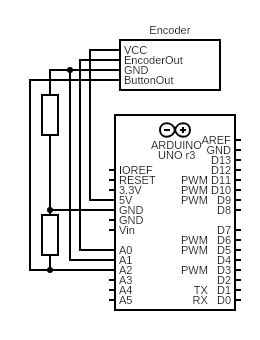
\includegraphics[width = \textwidth]{Documentation Assets/CircuitDiagramModular.png}
                    \caption{Circuit Diagram}
                \end{minipage} \hfill
                \begin{minipage}[b]{0.45\textwidth}
                    \centering
                    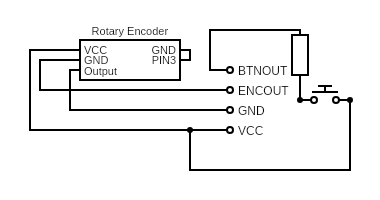
\includegraphics[angle = -90, width = 0.8\textwidth]{Documentation Assets/EncoderPCB.png}
                    \caption{Circuit Diagram}
                \end{minipage} \hfill
            \end{figure}

            \subsubsection{Component List}
                \begin{itemize}
                    \item Arduino Uno
                    \item Rotary Encoder
                    \item Pull Down Resistor
                    \item Push-To-Make Button
                \end{itemize}
            

    \newpage

    \section{UML Diagrams}
    \begin{figure}[h!]
        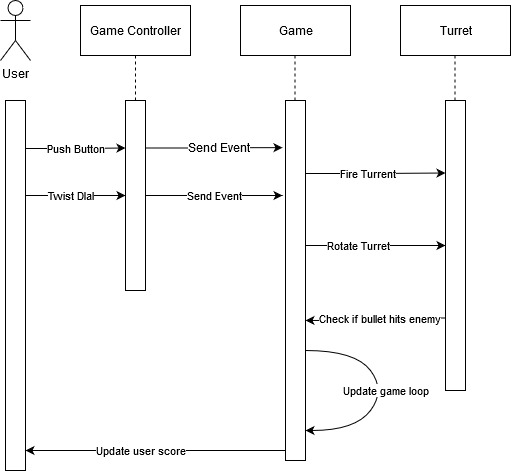
\includegraphics[width = \linewidth]{Documentation Assets/UML Diagrm.jpg}
        \caption{Use Case Diagram}
    \end{figure}

    \begin{figure}[h!]
        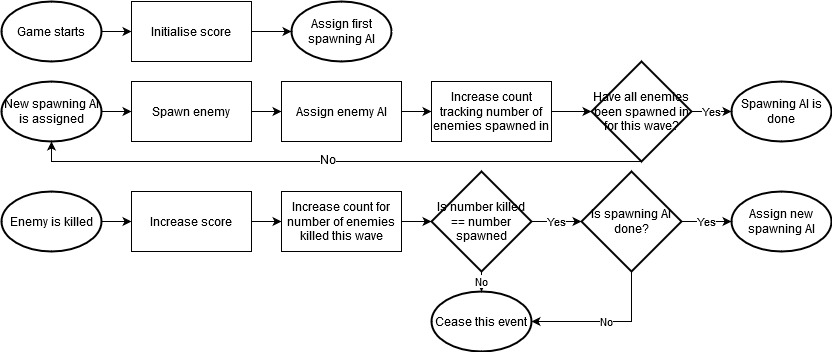
\includegraphics[width = \linewidth]{Documentation Assets/PhysicalControllerFlowChart2.jpg}
        \caption{Game Logic Flowchart}
    \end{figure}

    \begin{figure}[h!]
        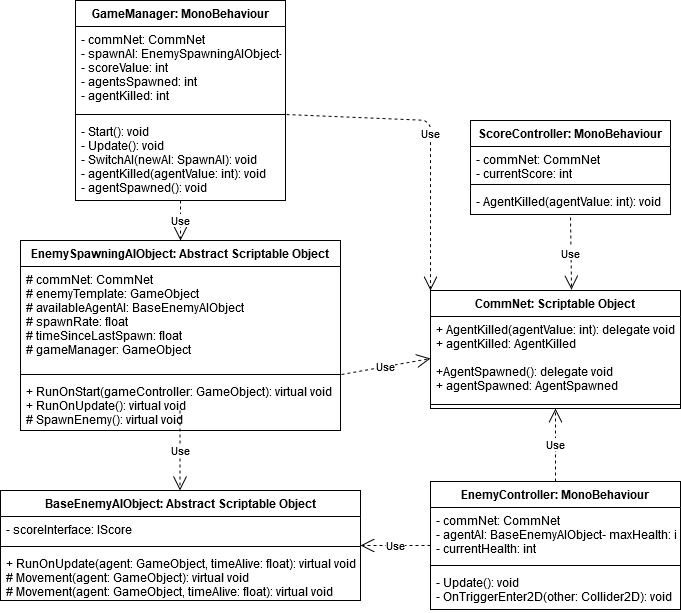
\includegraphics[width = \linewidth]{Documentation Assets/ClassDiagram.jpg}
        \caption{Class Diagram}
    \end{figure}

    \newpage

    \section{Reflection}
        \subsection{Concept}
            My initial concept idea, a choose your own adventure style game played using the same controller, with the text displayed on the vacuum fluorescent display, unfortunately had to be scrapped due to how the display was mounted to the PCB. This new concept was intentionally scaled back in order to allow more time to work on the GAM130 project, and has mostly been acting as a test bed for creating hot-swappable AI modules and using scriptable objects and delegates to make decoupled event driven systems. \\
            I have previously done electronics at GCSE, as such I've already been exposed to this style of project and have limited interest in the physical aspect. It has, however, provided a nice break and change of pace to our usual projects, and working on a physical piece can certainly be satisfying.

        \subsection{UML Diagrams}
            This was my first time really using UML diagrams, and I have actually found them very useful. While the user diagram was mostly unnecessary given the simplicity of the interactions, the class diagram proved very useful for planning out classes and seeing dependencies. This made it easy to see that there were a lot of interdependencies, and directly led to me implementing the CommNet scriptable object to fix this problem. I can see the use of these event systems leading to much cleaner code, with the planning that comes from creating a UML diagram being a big help.

        \subsection{Software}
            As mentioned above I have used this project to experiment with delegates and AI modules, neither of which I had done before. This project did lead to a 'eureka' moment when I finally understood what delegates actually were, whereupon I begun to realise just how useful they could be. \\
            I am also quite proud of the AI modules, while the actual AI is very simple, the framework I've built could easily be used in other projects. This could potentially form the basis for a finite state machine style AI and should make the assignment and management of sub and super states easier.

\end{document}